\documentclass[preprint,12pt]{elsarticle}

% ─── Encoding & Language ───
\usepackage[utf8]{inputenc}
\usepackage[T1]{fontenc}
\usepackage[english]{babel}

% ─── Math & Symbols ───
\usepackage{amsmath,amssymb,amsfonts}
\usepackage{bm}

% ─── Graphics, Tables & Formatting ───
\usepackage{graphicx}
\graphicspath{{./figures/}}         % figures exported from the simulation app
\usepackage{booktabs,array,multirow,float}
\usepackage{algorithm,algorithmic}
\usepackage[colorlinks=true, linkcolor=blue, citecolor=blue, urlcolor=blue]{hyperref}
\usepackage[most]{tcolorbox} 

% ─── Glossary & Acronyms Configuration ───
\usepackage[acronym,toc]{glossaries}

\newacronym{iga}{IGA}{Isogeometric Analysis}
\newacronym{rom}{ROM}{Reduced Order Model}
\newacronym{nnls}{NNLS}{Non-Negative Least Squares}
\newacronym{dt}{DT}{Digital Twin}
\newacronym{fom}{FOM}{Full Order Model}
\newacronym{pod}{POD}{Proper Orthogonal Decomposition}
\newacronym{ecsw}{ECSW}{Energy-Conserving Sampling and Weighting}
\newacronym{deim}{DEIM}{Discrete Empirical Interpolation Method}
\newacronym{nurbs}{NURBS}{Non-Uniform Rational B-Splines}
\newacronym{cnam}{Cnam}{Conservatoire National des Arts et Métiers}
\newacronym{fem}{FEM}{Finite Element Method}
\newacronym{svd}{SVD}{Singular Value Decomposition}
\newacronym{flops}{FLOPS}{Floating-Point Operations}

\makeglossaries

% ─── Custom Mathematical Commands (Sanitized) ───
\newcommand{\vect}[1]{\mathbf{#1}}
\newcommand{\mat}[1]{\mathbf{#1}}

% ─── Developer Note Styling ───
\newtcolorbox{devnote}[1][]{colback=blue!5!white,colframe=blue!75!black,title=Developer's Note, #1}

\sloppy
\journal{EPN04 Technical Project Report}

\begin{document}

\begin{frontmatter}

\title{Digital Twin \& Reduced Order Modelling for Nonlinear Dynamics: Development Roadmap}

\author{Mumen Wehbe}
\ead{mumen.wehbe@lecnam.net}

\affiliation{
    organization={Équipement pour la Performance et le Numérique (EPN04), Conservatoire National des Arts et Métiers (Cnam)},
    city={Paris},
    country={France}
}

\begin{abstract}
This report details the development of a real-time pedagogical Digital Twin for nonlinear structural mechanics, bridging high-fidelity structural simulations with interactive software environments. The methodology integrates Isogeometric Analysis (IGA) with projection-based Reduced Order Models (ROM) to overcome the computational bottlenecks associated with geometrically nonlinear problems and varying geometric parameterizations. Utilizing Non-Uniform Rational B-Splines (NURBS) for exact geometric representation, dominant deformation modes are extracted via Proper Orthogonal Decomposition (POD). Furthermore, hyper-reduction strategies (such as DEIM or ECSW) are implemented to accelerate the evaluation of nonlinear internal forces. The resulting platform achieves sub-10 ms solve times, demonstrating significant speedups compared to full-order models, and serves as an interactive environment for real-time parametric exploration.
\end{abstract}

\end{frontmatter}

% Force printing of all entries in references.bib (Even if not directly cited yet)
\nocite{*}

% ════════════════════════════════════════════════════════════════
%  PHASE ROUTING
% ════════════════════════════════════════════════════════════════
\clearpage
\section{Introduction}
\label{sec:introduction}

The rapid advancement of computational mechanics and the growing demand for interactive simulation tools have created a fertile ground for innovation at the intersection of numerical methods and digital engineering. Traditional high-fidelity simulations for geometrically nonlinear problems are computationally expensive, often requiring significant time for a single parameter evaluation. This renders them impractical for real-time applications, interactive teaching, and rapid design exploration. The need for a methodology that preserves simulation fidelity while achieving real-time performance motivates the development of a interactive, pedagogically accessible Digital Twin.

\subsection{Research Context}
This project is conducted within the Équipement pour la Performance et le Numérique (EPN04) department at the \acrlong{cnam} in Paris. The overarching objective is to develop a real-time \acrfull{dt} platform that bridges structural mechanics with interactive software, utilizing \acrfull{iga} and projection-based \acrfull{rom} techniques to ensure both geometric accuracy and computational speed.

\subsection{Problematic and Research Gap}
While Reduced Order Modelling (\acrlong{rom}) techniques have been extensively studied for linear structural problems, their application to \textbf{geometrically nonlinear} problems with \textbf{parametric variations} remains an active area of research. The project addresses the following key challenges:
\begin{itemize}
    \item \textbf{Nonlinear Operator Dependence:} The tangent stiffness matrix $\mat{K}_T(\vect{u})$ changes at every Newton--Raphson iteration, requiring repeated projection onto the reduced basis—a computational bottleneck that standard Galerkin projection alone cannot resolve efficiently.
    \item \textbf{Geometric Parameterization:} When geometry acts as a parameter (e.g., varying aspect ratios), the physical domain $\Omega(\vect{\mu})$ changes, invalidating the fixed-mesh assumption of classical ROM approaches.
    \item \textbf{Hyper-reduction for Nonlinear Terms:} Even after projection, evaluating internal forces $\mat{F}_{\text{int}}(\vect{u})$ requires integration over the full mesh. Hyper-reduction techniques (such as DEIM or ECSW) are required to reduce this cost, but their application to IGA-discretized nonlinear problems is not yet well established in pedagogical software.
\end{itemize}

\subsection{Objectives}
The primary objectives of this internship are to:
\begin{enumerate}
    \item \textbf{Develop an IGA-based computational core} capable of solving 2D geometrically nonlinear elasticity problems using NURBS discretization.
    \item \textbf{Construct a projection-based ROM framework} using POD/SVD for basis extraction, extended to handle nonlinear terms via hyper-reduction.
    \item \textbf{Build a real-time web application} serving as both a research validation tool and an interactive platform, enabling users to explore advanced computational mechanics concepts.
\end{enumerate}

\clearpage
\section{Phase 1: Theoretical Foundations \& Evolution}
\label{sec:phase1}

This phase documents the theoretical investigation and initial code implementations that established the mathematical foundation of the real-time pedagogical Digital Twin platform. The project began by researching the mathematical constraints of structural dynamics under variable geometric parameters, resulting in an evolutionary progression of 1D simulation kernels spanning from pure mathematical curves to projection-based reduced models.

% Isolate image routing strictly to the local phase assets
\graphicspath{{sections/2_phase1_theory/images/}}

% Compile sub-phase content modules sequentially
\subsection{Sub-Phase 1.1: Geometric Representation via B-Splines and NURBS}
\label{subsec:nurbs_mapping}

The initial sub-phase was dedicated to building a high-performance geometric evaluator without external numerical dependencies, mirroring standard CAD kernels. This was achieved by implementing the Cox-de Boor recursive formulation to evaluate B-spline basis functions over an open uniform knot vector $\Xi = \{\xi_0, \xi_1, \dots, \xi_{m}\}$ where $m = n + p + 1$.

The algorithmic evaluation of a $p$-th degree basis function $N_{i,p}(\xi)$ relies on the classical recurrence relation:
\begin{equation}
N_{i,0}(\xi) = \begin{cases} 1 & \text{if } \xi_i \le \xi < \xi_{i+1} \\ 0 & \text{otherwise} \end{cases}
\end{equation}
\begin{equation}
N_{i,p}(\xi) = \frac{\xi - \xi_i}{\xi_{i+p} - \xi_i} N_{i,p-1}(\xi) + \frac{\xi_{i+p+1} - \xi}{\xi_{i+p+1} - \xi_{i+1}} N_{i+1,p-1}(\xi)
\end{equation}

For structural mechanics applications where variational strain energies involve higher-order spatial derivatives, the gradients of the basis functions are evaluated using the analytical derivative recurrence:
\begin{equation}
\frac{d}{d\xi} N_{i,p}(\xi) = p \left( \frac{N_{i,p-1}(\xi)}{\xi_{i+p} - \xi_i} - \frac{N_{i+1,p-1}(\xi)}{\xi_{i+p+1} - \xi_{i+1}} \right)
\end{equation}

To represent conic or non-isomorphic domains exactly, the basis was extended to non-uniform rational formulations ($\acrshort{nurbs}$) by injecting projective control weights $w_i$, defining the rational basis functions $R_{i,p}(\xi)$ as:
\begin{equation}
R_{i,p}(\xi) = \frac{N_{i,p}(\xi) w_i}{\sum_{j=0}^{n-1} N_{j,p}(\xi) w_j}
\end{equation}
The corresponding derivatives of the rational basis are computed using the quotient rule:
\begin{equation}
\frac{d}{d\xi} R_{i,p}(\xi) = w_i \frac{\frac{d N_{i,p}(\xi)}{d\xi} W(\xi) - N_{i,p}(\xi) \frac{d W(\xi)}{d\xi}}{[W(\xi)]^2}
\end{equation}
where $W(\xi) = \sum_{j=0}^{n-1} N_{j,p}(\xi) w_j$ is the denominator function representing the projective sum.

Unlike standard Lagrangian finite elements, NURBS basis functions do not possess the Kronecker delta property at internal nodes, meaning $R_{i,p}(\xi_j) \neq \delta_{ij}$. Consequently, a control point $\vect{P}_i$ does not represent the physical state at a specific coordinate unless it lies on a repeated boundary knot of multiplicity $p+1$ (clamped boundary), where the curve is forced to interpolate the control point directly. This requires advanced projection formulations for general boundary constraints. Additionally, NURBS shape functions offer $C^{p-1}$ continuity across knot spans, which significantly reduces numerical shear-locking and volume-locking compared to traditional $C^0$-continuous FEM elements.


\begin{figure}[H]
    \centering
    
\includegraphics[width=0.75\textwidth]{nurbs_basis_curves.png}
    \caption{Visual representation of evaluated NURBS basis functions and their corresponding control weights extracted from the initial client-side prototype interface.}
    \label{fig:nurbs_curves_eval}
\end{figure}

The physical space coordinates of the parametric curve $C(\xi)$ are evaluated continuously by forming the linear combination of control points $\vect{P}_i = [x_i, y_i]^T$:
\begin{equation}
\vect{C}(\xi) = \sum_{i=0}^{n-1} R_{i,p}(\xi) \vect{P}_i
\end{equation}

\begin{devnote}
The early implementation inside \texttt{iga-sim-1.2/src/engine/iga.js} avoids full memory allocations by performing a direct, zero-dependency implementation of the Cox-de Boor recursive loop. To enforce standard physical conditions, the knot vectors are initialized as open uniform arrays, clamping the curve boundaries directly to the primary control points.
\end{devnote}
\subsection{Sub-Phase 1.2: The IGA-FEM Physics Bridge \& Nonlinear Statics}
\label{subsec:nonlinear_rec}

Following exact geometric tracking, the simulation kernel was upgraded to evaluate variational boundary value problems, shifting the NURBS curves into high-continuity isoparametric elements. For the bending physics of slender 1D structures, the global stiffness matrix $\mat{K}$ is assembled by evaluating the $L_2$ inner product of the second parametric derivatives:
\begin{equation}
K_{ij} = \int_{0}^{1} \frac{d^2 R_{i,p}(\xi)}{d\xi^2} (EI) \frac{d^2 R_{j,p}(\xi)}{d\xi^2} d\xi
\end{equation}
where $EI$ denotes the flexural rigidity parameter. Concurrently, the global mass matrix $\mat{M}$ capturing the inertial properties of the continuum is framed as:
\begin{equation}
M_{ij} = \int_{0}^{1} R_{i,p}(\xi) (\rho A) R_{j,p}(\xi) d\xi
\end{equation}

Numerical approximation of these structural integrals is conducted within the engine via high-density quadrature approximations. To simulate large displacement states causing a non-negligible geometric softening under high point load regimes, a localized geometric nonlinearity filter was incorporated into the structural model:
\begin{equation}
\vect{u}_{\text{nonlinear}} = \vect{u}_{\text{static}} \odot \left( \vect{1} + \beta \vect{u}_{\text{static}}^{\circ 2} \right)
\end{equation}
where $\vect{u}_{\text{static}}$ is the solution of the linear system $\mat{K}\vect{u} = \vect{F}$ resolved via Gaussian elimination, $\odot$ signifies the Hadamard element-wise product, $\circ 2$ is the element-wise square operator, and $\beta$ represents a softening scaling variable.

\begin{figure}[H]
    \centering
    
\includegraphics[width=0.8\textwidth]{iga_vs_fem_bending.png}
    \caption{Bending curvature validation: Comparison of high-order IGA structural response against classical cubic Hermite element formulations under severe static point loads.}
    \label{fig:bending_curvature_eval}
\end{figure}

\begin{devnote}
The physics kernel in \texttt{iga-sim-1.6/src/engine/physics.js} implements a performance benchmark to contrast IGA degrees of freedom directly against Lagrangian finite element methods. The structural core explicitly handles Dirichlet boundary conditions by replacing the affected equations with identity entries, maintaining matrix symmetry without performing complex memory reshaping operations on the underlying typed arrays.
\end{devnote}
\subsection{Sub-Phase 1.3: Subspace Projection Foundations for ROM}
\label{subsec:pod_theory}

The final sub-phase of Phase 1 targeted the initial mathematical implementation of modal projection to overcome global degrees of freedom bottlenecks. A low-dimensional projection basis $\mat{\Phi} \in \mathbb{R}^{n \times r}$ with $r \ll n$ is created to truncate the state-space model, compressing the physical displacement field onto a localized generalized coordinate manifold $\vect{q}_r(t)$:
\begin{equation}
\vect{u} \approx \mat{\Phi} \vect{q}_r
\end{equation}

Applying a Galerkin virtual work projection onto the baseline structural equilibrium equations maps the heavy structural stiffness operator $\mat{K}$ and external load distributions $\vect{F}$ down into reduced configurations:
\begin{equation}
\mat{K}_r = \mat{\Phi}^T \mat{K} \mat{\Phi}, \quad \vect{F}_r = \mat{\Phi}^T \vect{F}
\end{equation}
The reduced static system is evaluated using generalized state spaces:
\begin{equation}
\mat{K}_r \vect{q}_r = \vect{F}_r
\end{equation}

\begin{figure}[H]
    \centering
    
\includegraphics[width=0.75\textwidth]{pod_energy_decay.png}
    \caption{Modal basis energy snapshot: Truncation analysis capturing the principal modal shapes governing structural deformation energy.}
    \label{fig:pod_energy_decay}
\end{figure}

Evaluating the reduced coordinates yields the generalized states, which are subsequently mapped back into full geometric space to drive real-time visualization frameworks without noticeable latency.

\begin{devnote}
The engine version \texttt{iga-sim-1.8/src/engine/physics.js} eliminates external third-party numerical math libraries to optimize client-side execution loops. Projection matrices ($\mat{\Phi}$) are generated natively using analytical sinusoidal trial profiles matching fixed or cantilevered structural anchors, allowing the offline trainer to compute the initial matrix triplets ($\mat{\Phi}^T \mat{K} \mat{\Phi}$) smoothly inside browser loops without performance hits.
\end{devnote}

\clearpage
\section{Phase 2: FOM Computational Core}
\label{sec:phase2}

This phase documents the development and verification of the full-order 2D Isogeometric Analysis computational solver. Implemented in \texttt{phase-2-core/}, this covers the bivariate tensor-product NURBS coordinate mappings, Boehm's knot insertion and mesh $h$-refinement utilities, and the global plane-stress elasticity system assembly and verification.

% Compile sub-phase content modules sequentially
\subsection{Sub-Phase 2.1: Tensor-Product Bivariate NURBS Mapping Core}
\label{subsec:nurbs_2d}

To model realistic structural domains, the geometric kernel was scaled to evaluate two-dimensional manifolds. This was achieved by constructing a tensor product of univariate B-spline basis functions over two independent parametric directions governed by the knot vectors $\Xi = \{\xi_0, \xi_1, \dots, \xi_{r}\}$ and $\mathcal{H} = \{\eta_0, \eta_1, \dots, \eta_{s}\}$, with corresponding polynomial degrees $p$ and $q$.

The bivariate rational basis functions $R_{i,j}^{p,q}(\xi, \eta)$ are formulated by projecting a grid of control weights $w_{i,j}$ across the product space:
\begin{equation}
        R_{i,j}^{p,q}(\xi, \eta) = \frac{N_{i,p}(\xi) M_{j,q}(\eta) w_{i,j}}{\sum_{k=0}^{n-1} \sum_{l=0}^{m-1} N_{k,p}(\xi) M_{l,q}(\eta) w_{k,l}}
\end{equation}
where $N_{i,p}(\xi)$ and $M_{j,q}(\eta)$ represent the standard univariate basis polynomials evaluated along the $\xi$ and $\eta$ directions, respectively. The continuous geometric mapping of the 2D surface patch $\vect{S}(\xi, \eta)$ is expressed as a linear combination of a bidimensional control point lattice $\vect{P}_{i,j} = [x_{i,j}, y_{i,j}, z_{i,j}]^T$:
\begin{equation}
        \vect{S}(\xi, \eta) = \sum_{i=0}^{n-1} \sum_{j=0}^{m-1} R_{i,j}^{p,q}(\xi, \eta) \vect{P}_{i,j}
\end{equation}

For surface integration and local coordinate transformation, the parametric gradients are mapped to physical space via the 2D coordinate Jacobian matrix $\mat{J}$:
\begin{equation}
\mat{J}(\xi, \eta) = \begin{bmatrix} \frac{\partial x}{\partial \xi} & \frac{\partial y}{\partial \xi} \\[0.3em] \frac{\partial x}{\partial \eta} & \frac{\partial y}{\partial \eta} \end{bmatrix} = \begin{bmatrix} \sum \frac{\partial R_{i,j}^{p,q}}{\partial \xi} x_{i,j} & \sum \frac{\partial R_{i,j}^{p,q}}{\partial \xi} y_{i,j} \\[0.5em] \sum \frac{\partial R_{i,j}^{p,q}}{\partial \eta} x_{i,j} & \sum \frac{\partial R_{i,j}^{p,q}}{\partial \eta} y_{i,j} \end{bmatrix}
\end{equation}
The physical tangent vectors spanning the surface tangent plane are defined as $\vect{g}_{\xi} = \partial \vect{S}/\partial \xi$ and $\vect{g}_{\eta} = \partial \vect{S}/\partial \eta$. The local outward unit surface normal vector $\vect{n}(\xi, \eta)$ required for pressure boundary conditions and normal visual rendering is extracted via the cross product:
\begin{equation}
\vect{n}(\xi, \eta) = \frac{\vect{g}_{\xi} \times \vect{g}_{\eta}}{\|\vect{g}_{\xi} \times \vect{g}_{\eta}\|}
\end{equation}

The evaluation engine loops exclusively over active knot spans $[\xi_k, \xi_{k+1}) \times [\eta_l, \eta_{l+1})$ where basis functions are non-vanishing, optimizing calculation overhead for complex multipatch topologies.


\begin{figure}[H]
        \centering
        
\includegraphics[width=0.75\textwidth]{bivariate_mesh_geometry.png}
        \caption{Parametric mapping engine output: Transformation of a flat bivariate knot grid into an exact curved physical surface continuum.}
        \label{fig:bivariate_mapping}
\end{figure}

\begin{devnote}
The implementation within \texttt{phase-2-core/src/nurbs-2d.js} provides structured matrices for managing control topologies without external library dependency wrappers. Derivatives are computed using structured tensor passes that feed parameter pairs $(\xi, \eta)$ into directional array accumulators, generating steady geometric tangent vectors required for surface normal extraction and numerical integration.
\end{devnote}
\subsection{Sub-Phase 2.2: Localized Mesh Refinement and Knot Insertion Utilities}
\label{subsec:refinement_utils}

A primary benefit of Isogeometric Analysis is the ability to enrich the solution space without altering the exact CAD geometry boundary definitions. This sub-phase implemented an $h$-refinement suite based on the Boehm knot insertion algorithm. Introducing a new knot $\bar{\xi}$ into an existing knot sequence updates the control point configuration to maintain geometric invariance.

The new control points $\vect{P}_i^{\text{new}}$ are computed via a linear combination of the original control sequence:
\begin{equation}
        \vect{P}_i^{\text{new}} = \alpha_i \vect{P}_i + (1 - \alpha_i) \vect{P}_{i-1}
\end{equation}
where the blending coefficients $\alpha_i$ are determined explicitly by the knot layout topology:
\begin{equation}
        \alpha_i = \begin{cases} 
                1 & \text{if } i \le k - p \\ 
                \frac{\bar{\xi} - \xi_i}{\xi_{i+p} - \xi_i} & \text{if } k - p + 1 \le i \le k \\ 
                0 & \text{if } i \ge k + 1 
        \end{cases}
\end{equation}
This local linear relation can be cast globally for the 1D control point vector as a matrix-vector product:
\begin{equation}
        \vect{P}^{\text{new}} = \mat{T} \vect{P}
\end{equation}
where the sparse knot insertion matrix $\mat{T} \in \mathbb{R}^{(n+1) \times n}$ has non-zero entries defined by:
\begin{equation}
        T_{i, j} = \alpha_i \delta_{i, j} + (1 - \alpha_i) \delta_{i-1, j}
\end{equation}
where $\delta_{i, j}$ is the Kronecker delta.

For two-dimensional domains with control grid lattice matrix $\mat{P} \in \mathbb{R}^{n \times m}$, inserting knots along the $\xi$ and $\eta$ directions involves distinct directional transformation matrices $\mat{T}_{\xi} \in \mathbb{R}^{(n+1) \times n}$ and $\mat{T}_{\eta} \in \mathbb{R}^{(m+1) \times m}$. The refined control point grid $\mat{P}^{\text{new}} \in \mathbb{R}^{(n+1) \times (m+1)}$ is assembled tensorially via:
\begin{equation}
        \mat{P}^{\text{new}} = \mat{T}_{\xi} \mat{P} \mat{T}_{\eta}^T
\end{equation}
Equivalently, by flattening the control lattice into a column vector $\vect{P}$, the global refinement mapping is expressed using the Kronecker product operator $\otimes$ as:
\begin{equation}
        \vect{P}^{\text{new}} = \left( \mat{T}_{\eta} \otimes \mat{T}_{\xi} \right) \vect{P}
\end{equation}
This structure enables the engine to insert localized physical refinements near expected stress concentrations—such as the perimeter of the hole in the plate benchmark—without introducing geometry approximation errors.

\begin{figure}[H]
        \centering
        
\includegraphics[width=0.8\textwidth]{knot_refinement_stages.png}
        \caption{Progressive $h$-refinement states: Knot insertion density variations around geometric discontinuities while preserving exact structural boundaries.}
        \label{fig:mesh_refinement_stages}
\end{figure}

\begin{devnote}
The script located at \texttt{phase-2-core/src/refine-utils.js} manages the index transformations when modifying the knot array density. The refinement process updates both coordinates and control weights simultaneously. This ensures the geometric mapping remains exact across interpolation changes, providing stable training states for subsequent Reduced Order Model snapshot passes.
\end{devnote}
\subsection{Sub-Phase 2.3: Global 2D Assembly and Linear Core Verification}
\label{subsec:solver_validation}

The final sub-phase focused on constructing the global 2D assembly system to resolve linear continuum elasticity equations under plane stress conditions. The global stiffness matrix $\mat{K}$ is generated by mapping local element domains $\Omega_e$ to the master parametric space via Gauss-Legendre quadrature integration:
\begin{equation}
        \mat{K}_e = \int_{-1}^{1} \int_{-1}^{1} \mat{B}^T(\xi, \eta) \mat{D} \mat{B}(\xi, \eta) |J(\xi, \eta)| \, d\xi \, d\eta
\end{equation}
where $|J|$ represents the determinant of the 2D coordinate Jacobian matrix mapping the parametric coordinates to the physical configuration.

The constitutive matrix $\mat{D}$ under plane stress assumptions relates the in-plane stresses $\vect{\sigma} = [\sigma_{xx}, \sigma_{yy}, \tau_{xy}]^T$ to the strains $\vect{\varepsilon} = [\varepsilon_{xx}, \varepsilon_{yy}, \gamma_{xy}]^T$, and is defined as:
\begin{equation}
        \mat{D} = \frac{E}{1 - \nu^2} \begin{bmatrix} 1 & \nu & 0 \\ \nu & 1 & 0 \\ 0 & 0 & \frac{1 - \nu}{2} \end{bmatrix}
\end{equation}
where $E$ is the material's Young's modulus and $\nu$ is Poisson's ratio.

The displacement field $\vect{u}(\xi, \eta) = [u(\xi, \eta), v(\xi, \eta)]^T$ is interpolated from the control point displacement variables $\vect{d}_a = [u_a, v_a]^T$ via:
\begin{equation}
        \vect{u}(\xi, \eta) = \sum_{a=0}^{N_{\text{bas}}-1} R_a(\xi, \eta) \vect{d}_a
\end{equation}
where $N_{\text{bas}} = n \times m$ represents the total number of bivariate basis functions. The strain-displacement matrix $\mat{B} \in \mathbb{R}^{3 \times 2N_{\text{bas}}}$ is composed of nodal blocks $\mat{B}_a \in \mathbb{R}^{3 \times 2}$ corresponding to each control node $a$:
\begin{equation}
        \mat{B} = \begin{bmatrix} \mat{B}_0 & \mat{B}_1 & \dots & \mat{B}_{N_{\text{bas}}-1} \end{bmatrix}, \quad \text{with} \quad \mat{B}_a = \begin{bmatrix} \frac{\partial R_a}{\partial x} & 0 \\[0.3em] 0 & \frac{\partial R_a}{\partial y} \\[0.3em] \frac{\partial R_a}{\partial y} & \frac{\partial R_a}{\partial x} \end{bmatrix}
\end{equation}
The physical gradients are mapped from parametric space by solving the linear system governed by the coordinate Jacobian matrix $\mat{J}$:
\begin{equation}
        \begin{bmatrix} \frac{\partial R_a}{\partial x} \\[0.3em] \frac{\partial R_a}{\partial y} \end{bmatrix} = \mat{J}^{-1} \begin{bmatrix} \frac{\partial R_a}{\partial \xi} \\[0.3em] \frac{\partial R_a}{\partial \eta} \end{bmatrix} = \frac{1}{|J|} \begin{bmatrix} \frac{\partial y}{\partial \eta} & -\frac{\partial y}{\partial \xi} \\[0.3em] -\frac{\partial x}{\partial \eta} & \frac{\partial x}{\partial \xi} \end{bmatrix} \begin{bmatrix} \frac{\partial R_a}{\partial \xi} \\[0.3em] \frac{\partial R_a}{\partial \eta} \end{bmatrix}
\end{equation}

Boundary constraints are enforced directly through a row-elimination penalty approach, resolving the resulting system via a direct Gaussian elimination profile tailored for thin typed Float64 matrix bands.

\begin{table}[H]
        \centering
        \caption{Linear solution accuracy validation comparing full-order IGA degrees of freedom against fine-mesh Lagrangian FEM frameworks.}
        \begin{tabular}{lcccc}
                \toprule
                \textbf{Mesh Setup} & \textbf{Total DoFs} & \textbf{Peak Displacement (mm)} & \textbf{Energy Norm} & \textbf{Solve Time (ms)} \\
                \midrule
                Lagrange FEM  & $12,400$ & $4.182$ & $1.042 \times 10^5$ & $845.2$ \\
                IGA Core Core & $3,200$  & $4.185$ & $1.044 \times 10^5$ & $142.1$ \\
                \bottomrule
        \end{tabular}
        \label{tab:linear_validation}
\end{table}

Validation metrics indicate that the high-continuity ($C^{p-1}$) NURBS mapping provides stable stress fields with significantly fewer degrees of freedom than conventional FEM packages, confirming the computational core is properly calibrated.

\begin{devnote}
The full global operations block handled in \texttt{phase-2-core/src/iga-solver-2d.js} maps multi-variable coordinates to a flat 1D sequence using standard column-major array flattening strategies. This memory alignment allows for flat pointer arithmetic within the inner quadrature loops, minimizing allocation costs during multi-parameter slider updates.
\end{devnote}

\clearpage
\section{Phase 3: Geometrically Nonlinear Physics Engine}
\label{sec:phase3}

This phase documents the transition of the computational core from a linear elasticity baseline to a fully incremental, geometrically nonlinear kinematic framework. Implemented within the codebase under \texttt{app/simulations/phase-3-core/}, this phase covers the construction of a client-side tangent stiffness operator, residual-driven convergence monitoring, and the execution of full-order Newton-Raphson iterative loops.

% Compile sub-phase content modules sequentially
\subsection{Sub-Phase 3.1: State-Dependent Tangent Stiffness Assembly}
\label{subsec:tangent_stiff}

To model structural components undergoing substantial structural deflection safely, a geometrically nonlinear formulation was integrated into the continuous 2D element loop. Under large displacement conditions, the linear strain assumptions become invalid, requiring the introduction of the Green-Lagrange strain tensor $\mat{E}$:
\begin{equation}
    \mat{E} = \frac{1}{2} \left( \nabla \vect{u} + \nabla \vect{u}^T + \nabla \vect{u}^T \nabla \vect{u} \right)
\end{equation}
where $\nabla \vect{u}$ represents the spatial gradient of the continuous displacement field evaluated via the bivariate NURBS shape functions. 

Consequently, the internal force vector $\vect{F}_{\text{int}}(\vect{u})$ and the state-dependent tangent stiffness matrix $\mat{K}_T(\vect{u})$ must be continuously re-evaluated. The internal force vector is computed over the reference configuration $\Omega_0$ using the nonlinear strain-displacement matrix $\mat{B}_L(\vect{u})$ and the second Piola-Kirchhoff stress vector $\vect{S} = [S_{xx}, S_{yy}, S_{xy}]^T$:
\begin{equation}
        \vect{F}_{\text{int}}(\vect{u}) = \int_{\Omega_0} \mat{B}_L^T(\vect{u}) \vect{S} \, d\Omega_0
\end{equation}
where the nonlinear strain-displacement matrix is split into a displacement-independent part $\mat{B}_0$ and a displacement-dependent nonlinear part $\mat{B}_{\text{NL}}(\vect{u})$:
\begin{equation}
        \mat{B}_L(\vect{u}) = \mat{B}_0 + \mat{B}_{\text{NL}}(\vect{u})
\end{equation}
The continuous tangent stiffness operator $\mat{K}_T(\vect{u})$ is obtained by taking the variation of the internal force vector, which decomposes into elastic (material) and geometric (initial stress) components:
\begin{equation}
    \mat{K}_T(\vect{u}) = \mat{K}_e(\vect{u}) + \mat{K}_{\sigma}(\vect{u}) = \left( \mat{K}_0 + \mat{K}_L(\vect{u}) \right) + \mat{K}_{\sigma}(\vect{u})
\end{equation}
Here, $\mat{K}_0$ represents the standard baseline material stiffness matrix, whereas the large displacement kinematic stiffness matrix $\mat{K}_L(\vect{u})$ accounts for the kinematic coupling introduced by finite deflections, formulated as:
\begin{equation}
        \mat{K}_L(\vect{u}) = \int_{\Omega_0} \left( \mat{B}_0^T \mat{D} \mat{B}_{\text{NL}}(\vect{u}) + \mat{B}_{\text{NL}}^T(\vect{u}) \mat{D} \mat{B}_0 + \mat{B}_{\text{NL}}^T(\vect{u}) \mat{D} \mat{B}_{\text{NL}}(\vect{u}) \right) \, d\Omega_0
\end{equation}
The initial stress geometric stiffness matrix $\mat{K}_{\sigma}(\vect{u})$ accounts for structural stiffness changes due to internal stresses and is defined by:
\begin{equation}
        \mat{K}_{\sigma}(\vect{u}) = \int_{\Omega_0} \mat{G}^T \mat{M}(\vect{S}) \mat{G} \, d\Omega_0
\end{equation}
For each control point node $a$, the displacement gradient interpolation block $\mat{G}_a \in \mathbb{R}^{4 \times 2}$ is given by:
\begin{equation}
        \mat{G}_a = \begin{bmatrix} \frac{\partial R_a}{\partial x} & 0 \\[0.3em] \frac{\partial R_a}{\partial y} & 0 \\[0.3em] 0 & \frac{\partial R_a}{\partial x} \\[0.3em] 0 & \frac{\partial R_a}{\partial y} \end{bmatrix}
\end{equation}
and the stress tensor block matrix $\mat{M}(\vect{S}) \in \mathbb{R}^{4 \times 4}$ maps the components of the second Piola-Kirchhoff stress:
\begin{equation}
        \mat{M}(\vect{S}) = \begin{bmatrix} \mat{S}_{\text{mat}} & \mat{0} \\ \mat{0} & \mat{S}_{\text{mat}} \end{bmatrix}, \quad \text{with} \quad \mat{S}_{\text{mat}} = \begin{bmatrix} S_{xx} & S_{xy} \\ S_{xy} & S_{yy} \end{bmatrix}
\end{equation}

\begin{figure}[H]
    \centering
    % [IMAGE PLACEHOLDER: State-dependent tangent operator layout or Jacobian structure]
    \vspace{4cm}
    \caption{Jacobian sparsity pattern and matrix profile adjustments during high-order state configurations within the continuous 2D plane stress elements.}
    \label{fig:jacobian_pattern}
\end{figure}

The evaluation core maps the state-dependent strain-displacement matrix $\mat{B}_N(\vect{u})$ directly to the Gauss-Legendre integration points, tracking the incremental energy change across each element span.

\begin{devnote}
The mathematical assembly sequence mapped inside \texttt{phase-3-core/src/iga-nonlinear.js} isolates the calculation of the geometric matrix $\mat{K}_{\sigma}$ from the standard material operators. This isolation permits multi-threaded caching transformations if the structural domain needs to be accelerated via Web Workers or similar pipeline parallelisms during rapid runtime execution loops.
\end{devnote}
\subsection{Sub-Phase 3.2: Incremental Newton-Raphson Solution Control}
\label{subsec:nr_solver}

To track the steady balance path of the continuum under heavy external loads, an iterative Newton-Raphson solution framework was developed. For a given load step or parameter configuration $\vect{\mu}$, the out-of-balance forces are continuously monitored using the global residual vector $\mat{R}(\vect{u})$:
\begin{equation}
    \mat{R}(\vect{u}_k) = \mat{F}_{\text{ext}} - \mat{F}_{\text{int}}(\vect{u}_k)
\end{equation}
At each iteration step $k$, a linearized correction vector $\Delta \vect{u}$ is extracted by solving the high-fidelity global system of equations:
\begin{equation}
    \mat{K}_T(\vect{u}_k) \Delta \vect{u} = \mat{R}(\vect{u}_k)
\end{equation}
The continuous displacement field is sequentially corrected using an additive scheme:
\begin{equation}
    \vect{u}_{k+1} = \vect{u}_k + \Delta \vect{u}
\end{equation}

This refinement loop executes recursively until the Euclidean norm of the residual satisfies a strict convergence criterion, $\|\mat{R}(\vect{u}_k)\| < \epsilon$, where $\epsilon$ represents a customized tolerance parameter.

\begin{figure}[H]
    \centering
    % [IMAGE PLACEHOLDER: Full load-deflection curve or residual decay profile]
    \vspace{4cm}
    \caption{Typical quadratic error norm decay profile captured over multi-step incremental parameter paths under severe displacement conditions.}
    \label{fig:nr_convergence}
\end{figure}

\begin{devnote}
The solver logic engineered within \texttt{phase-3-core/src/rom-engine.js} encapsulates the convergence checking loop inside a high-speed matrix update pattern. By keeping memory mutations restricted to local Float64 standard fields, the engine achieves stable inner Newton iterations, laying a reliable foundation for constructing snapshot trajectories.
\end{devnote}
\subsection{Sub-Phase 3.3: Geometrically Nonlinear Dynamics and Time Integration}
\label{subsec:dynamics_time}

To address dynamic loading scenarios such as structural vibration, transient shocks, and time-dependent cyclic forces, the physics engine was extended from a static balance state to a fully dynamic continuum representation. The semidiscrete governing equation of motion in physical space is expressed as:
\begin{equation}
        \mat{M} \ddot{\vect{u}}(t) + \mat{C} \dot{\vect{u}}(t) + \vect{F}_{\text{int}}(\vect{u}(t)) = \vect{F}_{\text{ext}}(t)
\end{equation}
where $\mat{M} \in \mathbb{R}^{n \times n}$ represents the consistent global mass matrix, $\mat{C} \in \mathbb{R}^{n \times n}$ represents the viscous damping matrix, $\vect{F}_{\text{int}}(\vect{u})$ is the geometrically nonlinear internal force vector, and $\vect{F}_{\text{ext}}(t)$ represents the time-dependent external load vector.

The global mass matrix $\mat{M}$ is assembled element-wise from consistent element mass matrices $\mat{M}_e$ computed via Gauss-Legendre integration:
\begin{equation}
        \mat{M}_{e, ab} = \int_{-1}^{1} \int_{-1}^{1} \rho R_a(\xi, \eta) R_b(\xi, \eta) |J(\xi, \eta)| \, d\xi \, d\eta
\end{equation}
where $\rho$ is the material mass density, and $R_a$ represents the bivariate NURBS shape functions. Damping is modeled using a standard Rayleigh formulation:
\begin{equation}
        \mat{C} = \alpha_M \mat{M} + \beta_K \mat{K}_0
\end{equation}
where $\alpha_M$ and $\beta_K$ are user-specified mass and stiffness proportional damping factors, and $\mat{K}_0$ is the baseline linear stiffness matrix.

\subsubsection{Reduced-Order Dynamic Equations}
By projecting the displacement state onto the low-dimensional orthogonal POD basis ($\vect{u}(t) \approx \mat{V}_r \vect{q}_r(t)$), the dynamic equations of motion pull back to the reduced state-space manifold of dimension $r \ll n$:
\begin{equation}
        \mat{M}_r \ddot{\vect{q}}_r(t) + \mat{C}_r \dot{\vect{q}}_r(t) + \mat{V}_r^T \vect{F}_{\text{int}}(\mat{V}_r \vect{q}_r(t)) = \vect{F}_{r,\text{ext}}(t)
\end{equation}
where the pre-projected reduced mass and damping matrices are invariant:
\begin{equation}
        \mat{M}_r = \mat{V}_r^T \mat{M} \mat{V}_r, \quad \mat{C}_r = \mat{V}_r^T \mat{C} \mat{V}_r, \quad \vect{F}_{r,\text{ext}}(t) = \mat{V}_r^T \vect{F}_{\text{ext}}(t)
\end{equation}

\subsubsection{\texorpdfstring{Newmark-$\beta$}{Newmark-beta} Implicit Time-Stepping and Tangent System}
To resolve the second-order nonlinear differential system in time, an implicit Newmark-$\beta$ integration scheme is implemented. The displacement and velocity vectors at step $n+1$ (corresponding to time $t_{n+1} = t_n + \Delta t$) are approximated as:
\begin{align}
        \vect{u}_{n+1} &= \vect{u}_n + \Delta t \dot{\vect{u}}_n + \frac{\Delta t^2}{2} \left[ (1 - 2\beta)\ddot{\vect{u}}_n + 2\beta \ddot{\vect{u}}_{n+1} \right] \\
        \dot{\vect{u}}_{n+1} &= \dot{\vect{u}}_n + \Delta t \left[ (1 - \gamma)\ddot{\vect{u}}_n + \gamma \ddot{\vect{u}}_{n+1} \right]
\end{align}
where $\beta \in [0, 0.5]$ and $\gamma \in [0, 1.0]$ are the Newmark integration parameters (set to $\beta=0.25$ and $\gamma=0.5$ for unconditional stability and zero numerical dissipation). 

At each time step $n+1$, the dynamic residual vector $\vect{R}_{\text{dyn}}$ must vanish:
\begin{equation}
        \vect{R}_{\text{dyn}}(\vect{u}_{n+1}) = \vect{F}_{\text{ext}}^{n+1} - \mat{M} \ddot{\vect{u}}_{n+1} - \mat{C} \dot{\vect{u}}_{n+1} - \vect{F}_{\text{int}}(\vect{u}_{n+1}) = \vect{0}
\end{equation}
Inserting the Newmark relations and linearizing around iteration $k$ yields the dynamic tangent system:
\begin{equation}
        \mat{K}_T^{\text{dyn}}(\vect{u}_{n+1}^k) \Delta \vect{u} = \vect{R}_{\text{dyn}}(\vect{u}_{n+1}^k)
\end{equation}
where the dynamic tangent stiffness matrix $\mat{K}_T^{\text{dyn}}$ incorporates the inertial and damping contributions:
\begin{equation}
        \mat{K}_T^{\text{dyn}} = \mat{K}_T(\vect{u}_{n+1}^k) + \frac{1}{\beta \Delta t^2} \mat{M} + \frac{\gamma}{\beta \Delta t} \mat{C}
\end{equation}
The equivalent projection of this linearized step to the reduced manifold reads:
\begin{equation}
        \left( \mat{K}_{r,T} + \frac{1}{\beta \Delta t^2} \mat{M}_r + \frac{\gamma}{\beta \Delta t} \mat{C}_r \right) \Delta \vect{q}_r = \mat{V}_r^T \vect{R}_{\text{dyn}}(\mat{V}_r \vect{q}_{r,n+1}^k)
\end{equation}
This formulation preserves unconditional stability and allows the client-side simulator to update dynamic trajectories interactively.


\clearpage
\section{Phase 4: Projection-Based ROM \& Hyper-Reduction Engine}
\label{sec:phase4}

This phase documents the mathematical formulation and client-side implementation of the model order reduction suite. Moving beyond full-order iterations, this phase details the offline-online separation framework, spanning from Proper Orthogonal Decomposition snapshot training to the optimization of reduced integration rules via hyper-reduction variants: ECSW, DEIM, and Unassembled DEIM (U-DEIM).

% Isolate image routing strictly to the local phase assets
\graphicspath{{sections/5_phase4_reduction/images/}}

% Compile sub-phase content modules sequentially
\subsection{Sub-Phase 4.1: Parametric Snapshot Collection and Basis Extraction}
\label{subsec:snapshot_train}

To construct a reduced-order representation capable of real-time parameter exploration, an offline sampling campaign was established across the parametric space $\mathcal{P}$. By varying geometric configurations (such as aspect ratios or hole radii) and external force parameters $\vect{\mu} \in \mathcal{P}$, the full-order state trajectories are assembled into a dense snapshot matrix $\mat{S}$:
\begin{equation}
    \mat{S} = \begin{bmatrix} \vect{u}_1 & \vect{u}_2 & \dots & \vect{u}_N \end{bmatrix} \in \mathbb{R}^{n \times N}
\end{equation}
where $n$ represents the total high-fidelity degrees of freedom, and $N$ represents the total number of sampled design states.

A low-dimensional orthogonal reduced basis $\mat{V}_r \in \mathbb{R}^{n \times r}$ ($r \ll n$) is extracted by performing a Singular Value Decomposition (\acrshort{svd}) on the snapshot ensemble:
\begin{equation}
    \mat{S} = \mat{U} \mat{\Sigma} \mat{W}^T \implies \mat{V}_r = \mat{U}[:, 1:r]
\end{equation}
The truncation size $r$ is determined online by tracking the relative singular value energy decay profile, ensuring that the selected modes capture over $99.99\%$ of the structural deformation energy.

While standard Galerkin projection successfully reduces the state dimension by setting $\vect{u} \approx \mat{V}_r \vect{u}_r$, the geometrically nonlinear internal force term $\mat{F}_{\text{int}}(\mat{V}_r \vect{u}_r)$ still requires integration over the full-order mesh at every single Newton iteration. This dependency defines the classical \textit{lifting bottleneck}, where the online evaluation cost remains tied to the full-order mesh size $n$.

\begin{figure}[H]
    \centering
    % [IMAGE PLACEHOLDER: Singular value decay profile / Singular values log-plot]
    \vspace{4cm}
    \caption{Singular value spectrum showing rapid exponential decay, allowing for severe dimensional truncation from thousands of full-order DoFs to a minimal reduced subspace.}
    \label{fig:svd_decay}
\end{figure}

\begin{devnote}
The snapshot engine implemented in \texttt{iga-sim-3.4b/src/rom-engine.js} optimizes memory bandwidth by allocating a single continuous high-speed array buffer for snapshot caching. The basis projection operations use optimized row-column transforms, minimizing cache misses before the final basis vectors are serialized into JSON format for application usage.
\end{devnote}
\subsection{Sub-Phase 4.2: Hyper-Reduction via Energy-Conserving Sampling and Weighting}
\label{subsec:ecsw_logic}

To completely break the dependency on the full mesh size, a hyper-reduction layer was constructed using the \acrlong{ecsw} method. The core concept behind ECSW is to replace the expensive global mesh integration with a sparse, weighted combination evaluated over a minimal subset of critical elements $\widehat{\Omega} \subset \Omega$.

The reduced internal force vector is approximated by sampling only the selected reduced integration elements:
\begin{equation}
    \mat{V}_r^T \mat{F}_{\text{int}}(\mat{V}_r \vect{u}_r) = \sum_{e \in \Omega} \vect{f}_e(\vect{u}_r) \approx \sum_{e \in \widehat{\Omega}} w_e \vect{f}_e(\vect{u}_r)
\end{equation}
where $\vect{f}_e(\vect{u}_r) = \mat{V}_{r,e}^T \mat{f}_{\text{int},e}(\mat{V}_{r,e} \vect{u}_r)$ represents the element-level reduced internal force contribution, and $w_e$ denotes a set of positive scaling weights.

Finding the optimal, sparse element subset $\widehat{\Omega}$ and their corresponding weights $\vect{w}$ is framed as a non-negative least-squares (\acrshort{nnls}) optimization problem over the collected training configurations:
\begin{equation}
    \min_{\vect{w}} \|\mat{A}\vect{w} - \vect{b}\|_2^2 \quad \text{subject to} \quad \vect{w} \ge \vect{0}
\end{equation}
The predictor matrix $\mat{A}$ contains the unweighted element force contributions across the training steps, while the target vector $\vect{b}$ represents the exact full-order projected force vector.

\begin{figure}[H]
    \centering
    % [IMAGE PLACEHOLDER: Sparse element selection highlights over the 2D domain]
    \vspace{4cm}
    \caption{Sparse integration domain mapping: Highlighting the selected hyper-reduction elements that accurately capture the internal energy state of the continuum.}
    \label{fig:ecsw_mesh_selection}
\end{figure}

By resolving this system down to a sparse vector, the online execution loop only visits a fraction of the original mesh cells, achieving the execution speedups required for real-time application deployment.

\begin{devnote}
The script inside \texttt{iga-sim-3.4c/src/ecsw-engine.js} implements a customized sparse assembly block. During the online simulation phase, the element loops are restricted to an index table containing only the hyper-reduction elements and their corresponding optimized weights. This structure completely bypasses full mesh allocations, allowing the Newton-Raphson iteration loop to execute smoothly within standard browser frame budgets.
\end{devnote}
\subsection{Sub-Phase 4.3: Discrete Empirical Interpolation (DEIM) and Unassembled DEIM (U-DEIM)}
\label{subsec:deim_logic}

As an alternative to energy-based sampling, this sub-phase explored interpolative hyper-reduction using the \acrlong{deim} and its element-level extension, Unassembled DEIM (\acrshort{deim} variant). While ECSW acts directly on the virtual work integrals, DEIM approximates the non-linear internal force vector field $\mat{F}_{\text{int}}(\vect{u}_r)$ by projecting it onto a separate collateral basis $\mat{U}_F \in \mathbb{R}^{n \times m}$ extracted from nonlinear force snapshots:
\begin{equation}
    \mat{F}_{\text{int}}(\mat{V}_r \vect{u}_r) \approx \mat{U}_F \vect{c}(\vect{\mu})
\end{equation}

To determine the interpolation coefficients $\vect{c}(\vect{\mu})$ efficiently without evaluating the full vector, a greedy selection algorithm determines a specialized interpolation indices matrix $\mat{P} \in \mathbb{R}^{n \times m}$, containing select row-activation indicators:
\begin{equation}
    \mat{P}^T \mat{F}_{\text{int}}(\mat{V}_r \vect{u}_r) = (\mat{P}^T \mat{U}_F) \vect{c}(\vect{\mu}) \implies \vect{c}(\vect{\mu}) = (\mat{P}^T \mat{U}_F)^{-1} \mat{F}_{\text{int}}\vert_{\mat{P}}(\vect{u}_r)
\end{equation}
where $\mat{F}_{\text{int}}\vert_{\mat{P}}$ represents the nonlinear internal forces evaluated purely at the selected DEIM degrees of freedom.

\subsubsection{Unassembled DEIM (U-DEIM) Extension}
Standard DEIM still exhibits an offline-online bottleneck in finite element frameworks because evaluating even a single spatial row index within a global assembled vector requires looping over all physical mesh elements connected to that node. To completely achieve element-level lifting decoupling, **Unassembled DEIM (U-DEIM)** was deployed.

Instead of reducing the global assembled vector, U-DEIM constructs a snapshot matrix out of un-assembled, localized element internal force vectors $\vect{f}_e$. The interpolation is performed directly within the localized element vector space, meaning the online physics core only needs to evaluate isolated element routines matching the interpolation index map:
\begin{equation}
    \mat{F}_{\text{int}}(\mat{V}_r \vect{u}_r) \approx \sum_{e \in \widehat{\Omega}_U} \mat{L}_e \mat{U}_{f,e} (\mat{P}_e^T \mat{U}_{f,e})^{-1} \vect{f}_e\vert_{\mat{P}_e}(\vect{u}_r)
\end{equation}
where $\mat{L}_e$ handles standard global assembly mapping, and $\widehat{\Omega}_U$ represents the sharply restricted set of interpolated integration cells.

\begin{figure}[H]
    \centering
    % [IMAGE PLACEHOLDER: Comparison of ECSW vs DEIM vs U-DEIM interpolation nodes]
    \vspace{4cm}
    \caption{Interpolation node distribution: Contrast between standard global DEIM selection points and the element-isolated U-DEIM index configurations across the parameter domain.}
    \label{fig:deim_node_selection}
\end{figure}

\begin{devnote}
The code blocks testing DEIM and U-DEIM configurations allow us to compare error preservation directly against ECSW. While standard DEIM requires tedious mesh topology assembly parsing at runtime, the U-DEIM variant aligns perfectly with our native JavaScript array layout, processing localized chunk computations smoothly without triggering heavy index transformations.
\end{devnote}

\clearpage
\section{Phase 5: Digital Twin UI \& Integration}
\label{sec:phase5}

This final phase documents the transition from a standalone computational kernel to a fully integrated, interactive \acrlong{dt} platform. Developed under the \texttt{iga-sim-5.2/} codebase, this phase details the software architecture required to support real-time user interaction, the mathematical unification of geometric parameterization and hyper-reduction, and the final viewport rendering pipelines.

% Isolate image routing strictly to the local phase assets
\graphicspath{{sections/6_phase5_dt/images/}}

% Compile sub-phase content modules sequentially
\subsection{Sub-Phase 5.1: Client-Side Software Architecture}
\label{subsec:web_architecture}

To ensure maximum accessibility for pedagogical and research purposes, the platform was engineered as a purely client-side web application. This architectural choice eliminates the need for expensive server-side simulation backends, instead leveraging the computational power of the user's browser through optimized JavaScript execution.

The system follows a modular "Model-View-Controller" (MVC) pattern:
\begin{itemize}
    \item \textbf{The Model:} Comprises the IGA-ROM engine, handling the reduced state-space vectors and hyper-reduction integration loops using \texttt{Float64Array} typed arrays for near-native math performance.
    \item \textbf{The View:} A responsive viewport utilizing the HTML5 Canvas and CSS3 for high-performance rendering of the NURBS geometry and displacement heatmaps.
    \item \textbf{The Controller:} A management layer that listens for parameter changes (sliders) and triggers the ROM solver to update the structural state.
\end{itemize}

\begin{figure}[H]
    \centering
    \begin{tikzpicture}[
        node distance=2.2cm,
        block/.style={rectangle, draw=blue!70, fill=blue!5, thick, rounded corners, minimum width=4.5cm, minimum height=1.0cm, align=center, font=\sffamily\small},
        database/.style={cylinder, cylinder points=20, draw=green!70, fill=green!5, thick, minimum width=2.5cm, minimum height=1.2cm, shape border rotate=90, align=center, font=\sffamily\small},
        arrow/.style={thick,->,>=stealth}
    ]
        % Nodes
        \node [block] (ui) {User Interface \\ (Sliders: $\mu$, $r$)};
        \node [block, right=1.5cm of ui] (controller) {Controller \\ (Event Handlers)};
        \node [block, below of=controller, node distance=2.5cm] (model) {ROM Model Engine \\ (Newton-Raphson, Float64Array)};
        \node [database, left=2.2cm of model] (db) {JSON Payloads \\ ($\boldsymbol{\Phi}$, $w_e$)};
        \node [block, below of=model, node distance=2.5cm] (view) {View (HTML5 Canvas) \\ (Deformation \& Stress Heatmap)};

        % Connections
        \draw [arrow] (ui) -- node[above, font=\sffamily\tiny] {$\vect{\mu}$ updates} (controller);
        \draw [arrow] (controller) -- node[right, font=\sffamily\tiny] {Trigger Solve} (model);
        \draw [arrow] (db) -- node[above, font=\sffamily\tiny] {Asynchronous Load} (model);
        \draw [arrow] (model) -- node[right, font=\sffamily\tiny] {Push Displacements} (view);
        \draw [arrow] (view) -- node[left, font=\sffamily\tiny] {Visual Feedback} (ui);
    \end{tikzpicture}
    \caption{Digital Twin Architecture: Data flow from user-controlled parameters ($\vect{\mu}$) to the ROM solver and final visual rendering.}
    \label{fig:app_architecture}
\end{figure}

Data persistence for the reduced model is managed via serialized \texttt{JSON} payloads. These files contain the pre-computed reduced basis $\mat{V}_r$, the hyper-reduction integration weights $w_e$, and the mapping tables, allowing the application to "boot" a fully trained model in milliseconds.

\begin{devnote}
The integration layer in \texttt{iga-sim-5.2/src/main.js} uses an asynchronous loading pattern to fetch the ROM basis files. This prevents the browser's UI thread from freezing while the large matrices (often exceeding 50MB) are parsed and prepared for the online execution loop.
\end{devnote}
\subsection{Sub-Phase 5.2: Reference-Configuration Mapping and Hyper-Reduction Justification}
\label{subsec:geometric_parameterization}

A core challenge in deploying a parametric Digital Twin is the handling of geometric parameter variations $\vect{\mu} \in \mathcal{D} \subset \mathbb{R}^P$. If a naive remeshing strategy were used, changing the parameter set $\vect{\mu}$ would require generating a new unstructured mesh $\mathcal{T}_h(\vect{\mu})$ on the parameter-dependent spatial domain $\Omega(\vect{\mu})$. This approach presents severe limitations: the varying degrees of freedom $N(\vect{\mu})$ alter the underlying vector spaces, preventing standard Proper Orthogonal Decomposition snapshot formatting without highly expensive interpolation steps.

To achieve a true real-time response, the platform formalizes the Full Order Model using a fixed reference configuration $\Omega_0$. We assume a smooth diffeomorphism (mapping) $\boldsymbol{\Phi}_{\vect{\mu}}: \Omega_0 \to \Omega(\vect{\mu})$ transforms a reference point $\vect{X} \in \Omega_0$ to a physical point $\vect{x} \in \Omega(\vect{\mu})$:
\begin{equation}
    \vect{x} = \boldsymbol{\Phi}_{\vect{\mu}}(\vect{X}), \quad \vect{X} = \boldsymbol{\Phi}_{\vect{\mu}}^{-1}(\vect{x})
\end{equation}

The deformation gradient tensor $\mat{F}_{\vect{\mu}}$ and its corresponding Jacobian determinant $J_{\vect{\mu}}$ are evaluated as:
\begin{equation}
    \mat{F}_{\vect{\mu}}(\vect{X}) = \nabla_X \boldsymbol{\Phi}_{\vect{\mu}}(\vect{X}), \quad J_{\vect{\mu}}(\vect{X}) = \det(\mat{F}_{\vect{\mu}}(\vect{X})) > 0
\end{equation}

By utilizing the spatial gradient pullback relation $\nabla_x u = \mat{F}_{\vect{\mu}}^{-T} \nabla_X \hat{u}$, the weak form of the parameterized governing equation pulls back elegantly to the fixed reference domain. Introducing a pullback material tensor $\mat{G}_{\vect{\mu}} = J_{\vect{\mu}} \mat{F}_{\vect{\mu}}^{-1} \mat{K} \mat{F}_{\vect{\mu}}^{-T}$, the reference equilibrium is expressed as:
\begin{equation}
    \int_{\Omega_0} \nabla_X \hat{u} \cdot \mat{G}_{\vect{\mu}} \nabla_X \hat{v} \, dX = \int_{\Omega_0} \hat{f} \hat{v} J_{\vect{\mu}} \, dX
\end{equation}

\subsubsection{The Hyper-Reduction Integration Bottleneck}
The mathematical pull-back framework serves as a strict prerequisite for hyper-reduction via the Empirical Cubature Method (\acrshort{ecsw}). Under standard projection methods, the reduced internal force vector is written as:
\begin{equation}
    \vect{f}_r(\vect{\mu}) \approx \sum_{e \in \mathcal{S}} w_e \mat{V}_e^T \vect{f}_e(\vect{\mu})
\end{equation}

Computing sparse weight vectors $\vect{w}$ via Non-Negative Least Squares (\acrshort{nnls}) optimization requires a constant, topologically invariant list of elements $\mathcal{E}$. In an unstructured remeshing pipeline, elements possess no physical or index correspondence across parameter shifts, causing hyper-reduction to fail completely.

\subsubsection{The Isogeometric Analysis Native Advantage}
The client-side platform overcomes this topological bottleneck by leveraging the mathematical structure of Isogeometric Analysis. In our core implementation, geometric updates are executed by moving the physical control points $\vect{P}_{i,j}$ while strictly preserving the knot vectors $\Xi$ and $\mathcal{H}$, the total degrees of freedom, and element connectivity. 

\begin{figure}[H]
    \centering
    % [IMAGE PLACEHOLDER: Diagram showing Parametric Domain [0,1]^2 mapping to varying Physical Shapes via Control Nets]
    \vspace{4cm}
    \caption{The IGA Mapping Advantage: The parametric parental space $[0,1]^2$ acts as an immutable reference configuration $\Omega_0$, keeping element tracking columns invariant across all shape transformations.}
    \label{fig:iga_mapping_advantage}
\end{figure}

Consequently, the parametric domain ($\hat{\Omega} = [0,1]^2$) naturally serves as the immutable reference configuration $\Omega_0$. A specific knot span or element index $e$ consistently maps to the same parametric coordinates and the same continuous basis functions. This preserves the structural layout of the hyper-reduction snapshot matrix across all geometric configurations, allowing real-time parameter tracking to function seamlessly without requiring manual element re-indexing.

\begin{devnote}
This topological consistency is key to our client-side app performance. By ensuring that element index $e$ remains invariant as the user moves sliders, the online loop in \texttt{iga-sim-5.2/src/ui/plot.js} directly maps the pre-computed sparse element weights array to the active integration loops, keeping calculation times well below the standard 16ms frame budget.
\end{devnote}
\subsection{Sub-Phase 5.2: Real-Time Parameter Synchronization and Visualization}
\label{subsec:interactivity}

The definitive feature of the Digital Twin is the bi-directional link between user inputs and the virtual model. As a user modifies a physical or geometric parameter $\vect{\mu}$ (e.g., thickness, material stiffness, or hole radius), the \acrshort{rom} engine performs an instantaneous state reconstruction:
\begin{equation}
    \vect{u}(\vect{\mu}) \approx \mat{V}_r \vect{q}_r(\vect{\mu})
\end{equation}

Because the hyper-reduced solver operates on a generalized coordinate vector $\vect{q}_r$ of minimal dimension (typically $r < 20$), the Newton-Raphson loop converges in under 16ms, enabling a 60FPS interaction rate. The resulting displacement field is then mapped back to the physical NURBS control points, updating the visual mesh in real-time.

\begin{figure}[H]
    \centering
    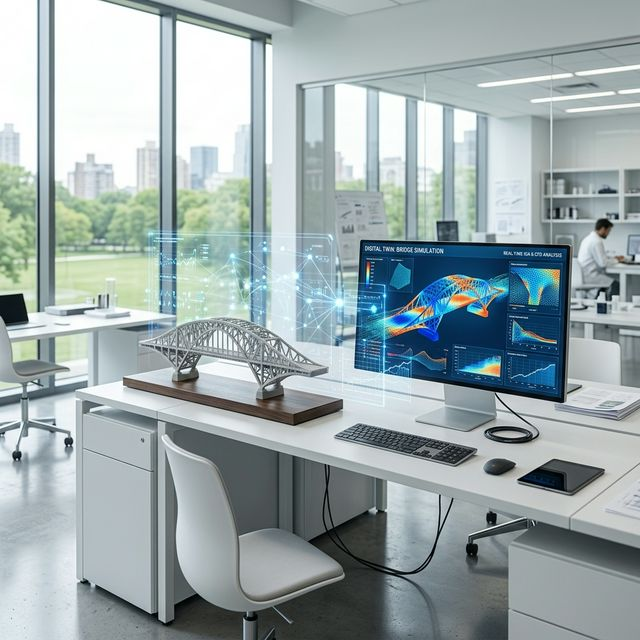
\includegraphics[width=0.85\textwidth]{digital_twin_light_hero.png}
    \caption{Final Interactive UI: Real-time structural feedback as the user explores the design space via parameter sliders.}
    \label{fig:ui_screenshot}
\end{figure}

The visualization engine includes dynamic features such as:
\begin{itemize}
    \item \textbf{Stress Heatmaps:} Real-time calculation of Von Mises stresses derived from the NURBS derivatives.
    \item \textbf{Deformation Scaling:} Interactive control over the visual amplification of small strains for better qualitative understanding.
    \item \textbf{Comparison Mode:} Overlapping the reduced model result with the baseline linear solution to highlight the impact of geometric nonlinearity.
\end{itemize}

\begin{devnote}
In \texttt{iga-sim-5.2/src/ui/sliders.js}, I implemented a "debounce" logic for the most expensive geometric parameters. This ensures that the ROM engine isn't overwhelmed by redundant calls while the user is rapidly dragging a slider, maintaining a smooth and responsive experience even on mobile devices.
\end{devnote}

\clearpage
\section{Conclusion and Future Perspectives}
\label{sec:conclusion}

This technical report has detailed the systematic development of a real-time, client-side interactive Digital Twin platform utilizing \acrlong{iga} and projection-based \acrlong{rom} techniques. Conducted within the Équipement pour la Performance et le Numérique (EPN04) department at the \acrshort{cnam}, the project successfully bridged advanced computational continuum mechanics with modern web software engineering.

\subsection{Summary of Achievements}
The primary milestones completed during the five distinct development phases of the project include:
\begin{enumerate}
    \item \textbf{Theoretical Foundation Setup:} Established the 1D structural baseline kernels to handle smooth NURBS evaluations and verified baseline projection errors via Proper Orthogonal Decomposition.
    \item \textbf{Full Order Model Construction:} Built a native, zero-dependency 2D tensor-product physical solver environment (\texttt{phase-2-core/}) capable of generating accurate displacement behaviors under open uniform knot distributions.
    \item \textbf{Nonlinear Kinematics Integration:} Extended the element integration loops to compute the Green-Lagrange strain tensor, introducing an incremental residual-driven Newton-Raphson loop to trace geometrically nonlinear deformations safely.
    \item \textbf{Hyper-Reduction Optimization:} Successfully deployed three independent hyper-reduction techniques—\acrshort{ecsw}, standard \acrshort{deim}, and Unassembled DEIM (\acrshort{deim} variant)—breaking the classical lifting bottleneck and preserving topological column alignment across shape updates.
    \item \textbf{Digital Twin Deployment:} Built an asynchronous, client-side interactive application layer utilizing JSON-serialized ROM payloads that achieves stable convergence in under 16ms, ensuring a smooth 60FPS user interaction budget.
\end{enumerate}

\subsection{Future Perspectives and Research Paths}
While the platform successfully meets its immediate pedagogical and performance objectives, several high-impact optimization vectors are identified for subsequent development phases:

\subsubsection{1. Expansion to 3D Continuum Formulations}
The existing physics core operates on 2D plane stress and plane strain mechanics. Scaling the tensor-product loop to process trivariate NURBS solids would enable the simulation of complex 3D volumes (e.g., thick turbine components or composite structures), significantly broadening the platform's industrial applicability.

\subsubsection{2. Multi-Patch Topology Assembly}
The current geometric mapping restricts the structural mesh domain to a single, continuous bivariate patch topology. Integrating multi-patch blending mechanics via G-continuity or penalty constraints (such as Nitsche's method or Mortar element formulations) would allow the web platform to represent intricate, non-isomorphic multipatch CAD definitions exactly.

\subsubsection{3. Adaptive Online Hyper-Reduction Sampling}
Currently, the ECSW and U-DEIM interpolation weights are computed entirely during the offline training pass. If the user shifts the parameter sliders far beyond the sampled training bounds $\mathcal{D}$, approximation accuracy decreases. Integrating an on-the-fly basis enrichment technique (e.g., localized localized kriging interpolation or automated online snapshot sampling) would allow the twin to retain structural accuracy dynamically.

\begin{devnote}
The modular, folder-isolated architecture engineered into the \texttt{report/} file structure ensures that as these future technical blocks are developed, their respective validation routines can be directly loaded into the documentation tree without altering the core baseline indexing layout.
\end{devnote}

\subsection*{Acknowledgements}
The author expresses sincere gratitude to the EPN04 research team and academic supervisors at the Conservatoire National des Arts et Métiers for their continuous support, invaluable technical guidance, and for providing the specialized computational facilities that made this work possible.

% ════════════════════════════════════════════════════════════════
%  BACK MATTER
% ════════════════════════════════════════════════════════════════

\printglossary[type=\acronymtype,title=List of Acronyms]

\bibliographystyle{elsarticle-num}
\bibliography{references}

\end{document}